\section{Results and Discussion}
\label{sec:results_discussion}

\subsection{Preliminary POD analysis using the 25-case dataset}
\label{subsec:preliminary_pod_results}

An initial POD analysis was performed using a training
dataset containing 25 full-order temperature solutions.
The dataset was generated from a uniform parameter grid
with five values of $\mu$ and five values of $Br$,
resulting in 25 parameter combinations. This preliminary
analysis was used to examine the dominant spatial modes
and assess how accurately the truncated POD basis
reconstructed the original training snapshots.

Figure~\ref{fig:initial_pod_modes} shows the first three
spatial POD modes obtained from the snapshot matrix.
These modes represent the dominant spatial patterns
extracted from the temperature-deviation fields through
singular value decomposition.

\begin{figure}[htbp]
    \centering
    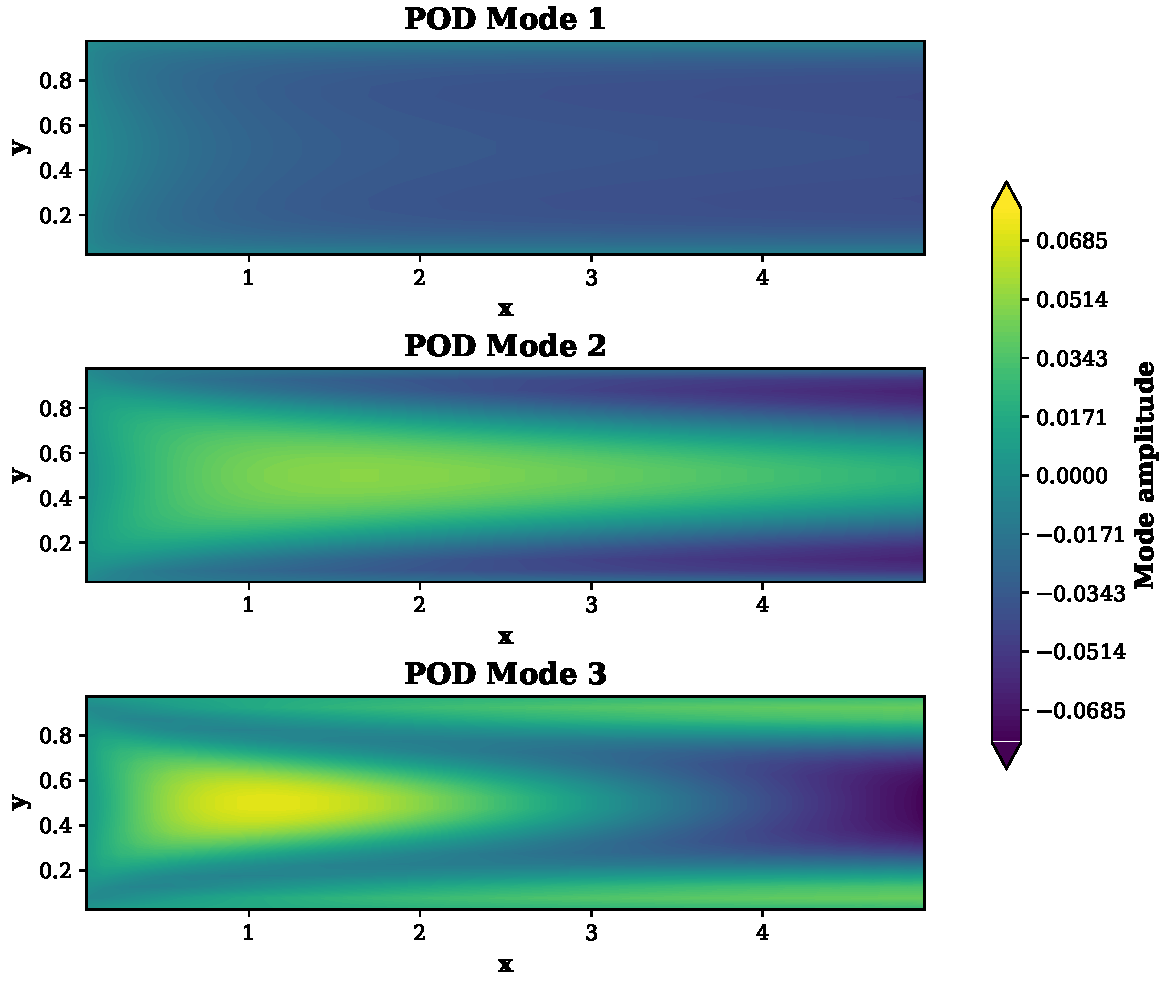
\includegraphics[width=0.95\textwidth]{figures/POD_modes.pdf}
    \caption{First three spatial POD modes obtained from
    the preliminary 25-snapshot dataset.}
    \label{fig:initial_pod_modes}
\end{figure}

The reconstruction accuracy was evaluated by projecting
the original snapshots onto the retained POD basis and
calculating the relative $L_2$ error for each case:
\begin{equation}
    \epsilon_k
    =
    \frac{
    \left\|
    \boldsymbol{\theta}_k
    -
    \hat{\boldsymbol{\theta}}_k
    \right\|_2
    }{
    \left\|
    \boldsymbol{\theta}_k
    \right\|_2
    },
    \label{eq:preliminary_pod_reconstruction_error}
\end{equation}
where $\boldsymbol{\theta}_k$ is the original
temperature-deviation snapshot and
$\hat{\boldsymbol{\theta}}_k$ is its POD reconstruction.
This measure evaluates the ability of the retained modes
to represent the snapshots used to construct the basis.

The reconstruction errors for the 25 cases are summarized
in Table~\ref{tab:preliminary_pod_errors}. Since the five
cases associated with each value of $\mu$ have identical
reported errors, the results are grouped according to
$\mu$ to avoid repeating the same values.

\begin{table}[htbp]
    \centering
    \caption{POD reconstruction errors for the preliminary
    25-case training dataset.}
    \label{tab:preliminary_pod_errors}
    \begin{tabular}{cccc}
        \toprule
        \textbf{$\mu$} &
        \textbf{Case IDs} &
        \textbf{$Br$ range} &
        \textbf{Relative $L_2$ error} \\
        \midrule
        1      & 1--5   & 0.01--2.00 & $4.96\times10^{-5}$ \\
        25.75  & 6--10  & 0.01--2.00 & $4.924\times10^{-3}$ \\
        50.50  & 11--15 & 0.01--2.00 & $1.7011\times10^{-2}$ \\
        75.25  & 16--20 & 0.01--2.00 & $3.284\times10^{-3}$ \\
        100    & 21--25 & 0.01--2.00 & $2.0632\times10^{-2}$ \\
        \bottomrule
    \end{tabular}
\end{table}

The minimum reconstruction error is
$4.96\times10^{-5}$, corresponding to cases 1--5
at $\mu=1$. The maximum error is
$2.0632\times10^{-2}$, corresponding to cases 21--25
at $\mu=100$. These values indicate that the
reconstruction accuracy varies across the sampled
values of $\mu$. The error does not increase
monotonically with $\mu$: it increases from the
lowest parameter value to $\mu=50.5$, decreases at
$\mu=75.25$, and reaches its maximum at $\mu=100$.

An additional observation is that the reconstruction
error remains identical across the five $Br$ values
for each fixed $\mu$. This behavior is consistent
with the linear structure of the steady reduced
governing equation. When the lifting residual is
zero or negligible, the temperature-deviation
equation has a source term proportional to $Br$.
Consequently, for a fixed $\mu$, the deviation
solutions scale linearly with $Br$. Both the
reconstruction error and the norm of the original
deviation field then scale proportionally, leaving
their relative ratio unchanged. The observed
repetition of the reconstruction errors across
different Brinkman numbers is consistent with
this property.

Figure~\ref{fig:preliminary_pod_reconstruction}
compares the full-order temperature fields, their
POD reconstructions, and the corresponding error
fields for representative minimum- and
maximum-error cases. Case 1 represents the
minimum-error group, while case 21 represents
the maximum-error group. Each of these cases has
the same reconstruction error as the other four
cases sharing its value of $\mu$.

\begin{figure}[htbp]
    \centering
    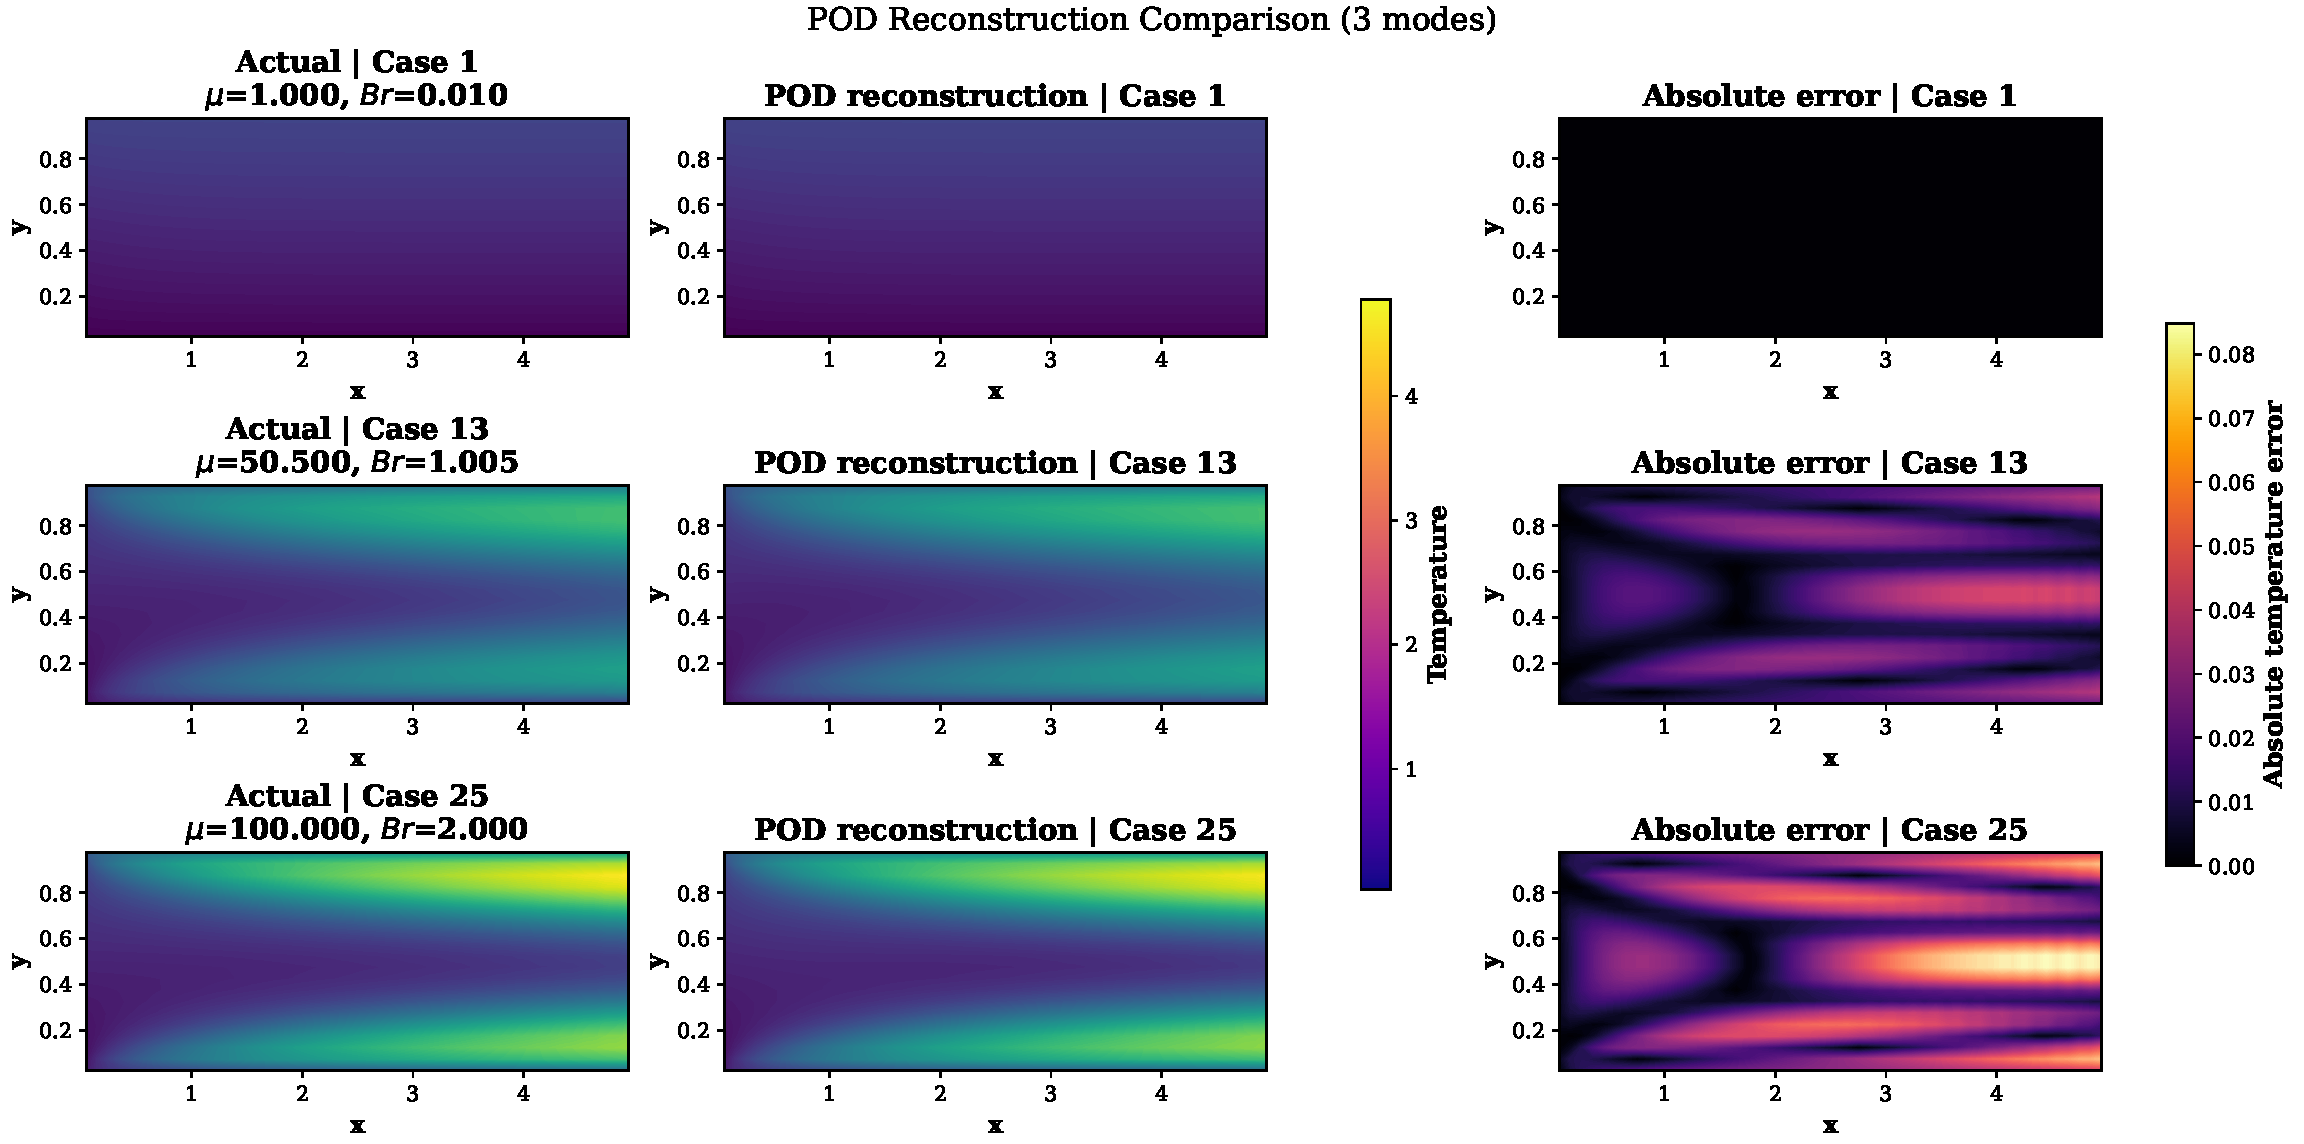
\includegraphics[width=\textwidth]
    {figures/POD_reconstruction.pdf}
    \caption{Comparison of the full-order temperature
    fields, POD reconstructions, and corresponding
    error fields for representative minimum-error
    and maximum-error cases from the preliminary
    25-case dataset.}
    \label{fig:preliminary_pod_reconstruction}
\end{figure}

The reconstruction plots provide a spatial comparison
of the original and approximated temperature fields.
The minimum-error case exhibits very close agreement
between the full-order and reconstructed fields,
whereas the maximum-error case has a larger
reconstruction discrepancy.

These results characterize the ability of the
initial POD basis to represent its own training
snapshots. They do not establish its accuracy at
parameter combinations outside the training dataset.
That question requires evaluating the reduced-order
model at independent parameter values, which is
examined in the following sections.

\subsection{Galerkin ROM results using the 100-snapshot POD basis}
\label{subsec:galerkin_rom_results}

The Galerkin reduced-order model was constructed using the
POD basis obtained from the 100 full-order training
solutions. As reported in Table~\ref{tab:pod_energy}, the
singular values exhibit a rapid decay. The first mode
accounts for 92.6360\% of the total snapshot energy, while
the first three modes capture 99.9833\%. Retaining four
modes increases the cumulative energy to 99.9995\%.

These results indicate that the training snapshots can
be represented using a relatively small number of spatial
modes. However, the accuracy of the Galerkin ROM also
depends on how well the reduced governing equations
determine the modal coefficients. Therefore, the ROM
temperature fields are compared directly with their
corresponding full-order solutions.

The ROM was evaluated for the 100 parameter combinations
in the original training dataset. For each case, the
Galerkin-projected system was solved, and the resulting
modal coefficients were used to reconstruct the complete
temperature field:
\[
\mathbf{T}_{\mathrm{ROM}}
=
\mathbf{T}_{\mathrm{ref}}+\mathbf{V}_r\mathbf{a}.
\]
The reconstructed fields were compared with the
corresponding full-order temperature solutions using
the relative discrete $L_2$ error, RMSE, and maximum
absolute error defined in the previous section.

The aggregate error statistics are reported in
Table~\ref{tab:initial_galerkin_errors}.

\begin{table}[htbp]
    \centering
    \caption{Aggregate Galerkin ROM errors over the
    100 training cases.}
    \label{tab:initial_galerkin_errors}
    \begin{tabular}{lc}
        \toprule
        \textbf{Metric} & \textbf{Value} \\
        \midrule
        Successful cases & 100 \\
        Mean relative $L_2$ error & $2.401402\times10^{-2}$ \\
        Median relative $L_2$ error & $1.705007\times10^{-2}$ \\
        Maximum relative $L_2$ error & $1.262083\times10^{-1}$ \\
        Mean RMSE & $6.498504\times10^{-2}$ \\
        Mean maximum absolute error & $1.353265\times10^{-1}$ \\
        \bottomrule
    \end{tabular}
\end{table}

The mean relative $L_2$ error across the 100 cases is
approximately 2.40\%, while the median error is
approximately 1.71\%. The maximum error reaches
approximately 12.62\%. The difference between the mean
and median indicates that the error distribution is
not uniform across the evaluated cases. Although most
cases have relatively small errors, some parameter
combinations produce considerably larger discrepancies.

The cases with the minimum and maximum relative
$L_2$ errors are summarized in
Table~\ref{tab:initial_galerkin_extremes}.

\begin{table}[htbp]
    \centering
    \caption{Minimum- and maximum-error cases in the
    initial Galerkin ROM evaluation.}
    \label{tab:initial_galerkin_extremes}
    \begin{tabular}{ccc}
        \toprule
        \textbf{Case} &
        \textbf{Relative $L_2$ error} &
        \textbf{Result} \\
        \midrule
        \texttt{train\_0001} &
        $7.040618\times10^{-6}$ &
        Minimum error \\
        \texttt{train\_0020} &
        $1.262083\times10^{-1}$ &
        Maximum error \\
        \bottomrule
    \end{tabular}
\end{table}

The minimum-error case has a relative $L_2$ error of
approximately $0.000704\%$, indicating very close
agreement between the full-order and reduced-order
temperature fields. In contrast, the maximum-error
case has a relative error of approximately 12.62\%.
This difference illustrates that the accuracy of the
reduced model varies across the parameter combinations,
even when the same POD basis and reduced formulation
are used.

Figures~\ref{fig:galerkin_minimum_error} and
\ref{fig:galerkin_maximum_error} present the spatial
comparison for the two cases. Each figure shows the
full-order temperature field, the reconstructed
Galerkin ROM temperature field, and their difference.

\begin{figure}[htbp]
    \centering
    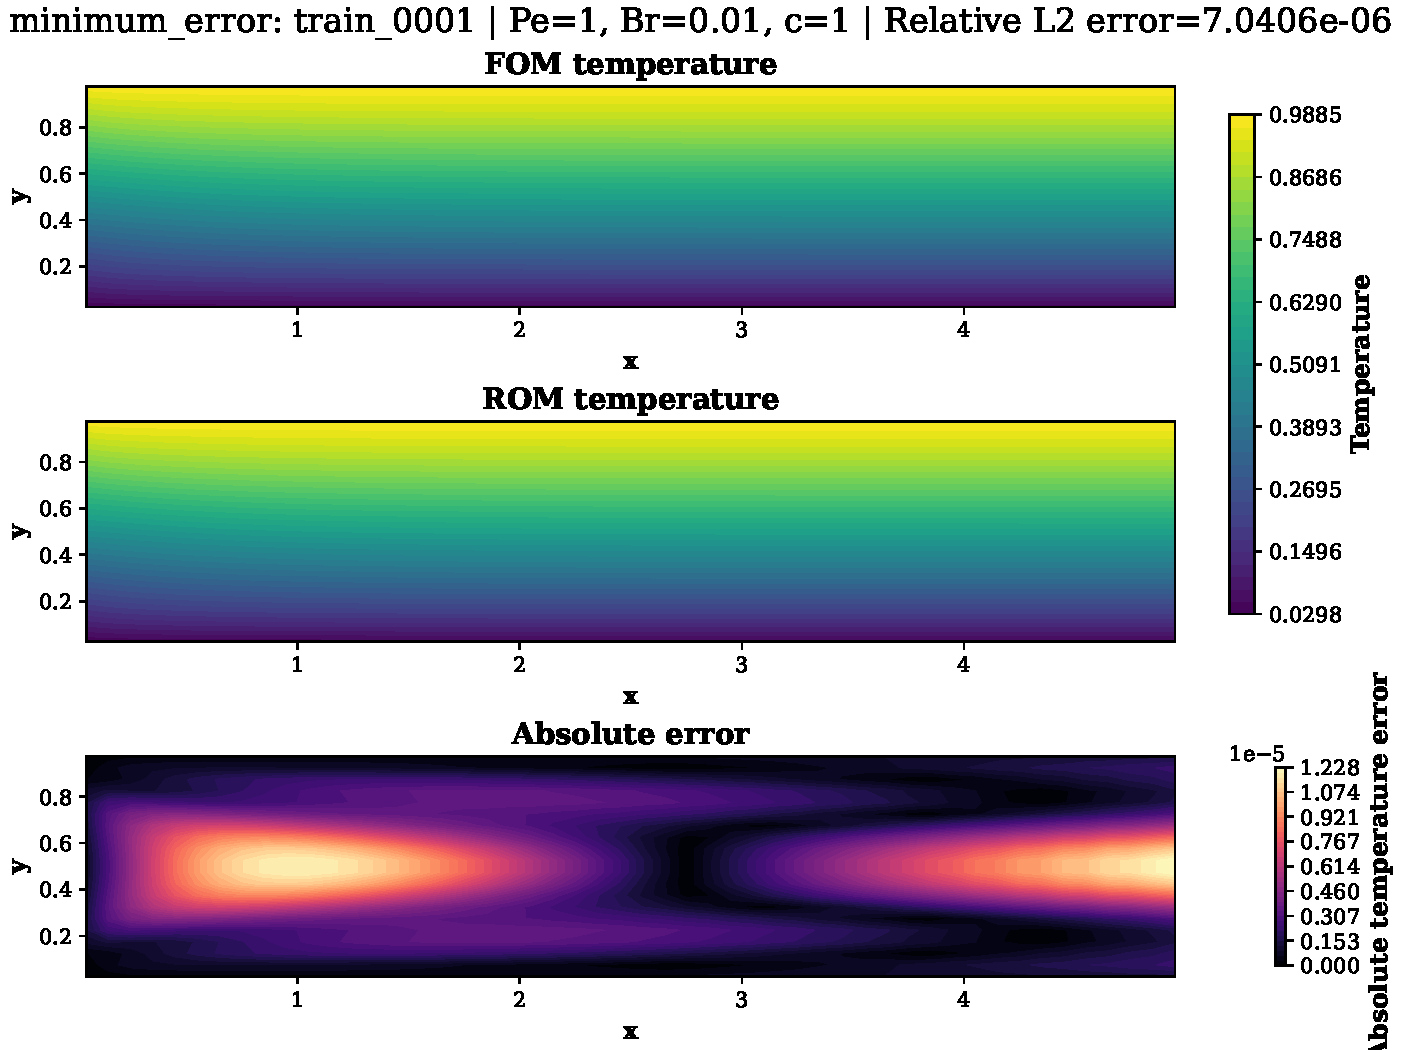
\includegraphics[width=\textwidth]
    {figures/Galerkin_minimum_error.pdf}
    \caption{Full-order temperature field, Galerkin ROM
    reconstruction, and corresponding error field for
    the minimum-error case (\texttt{train\_0001}).}
    \label{fig:galerkin_minimum_error}
\end{figure}

The comparison of the two cases provides a spatial
interpretation of the aggregate error statistics.
The minimum-error reconstruction exhibits close
agreement with the full-order solution, whereas the
maximum-error case displays larger discrepancies
between the two fields.

It should be noted that these 100 parameter combinations
were also used to construct the original POD basis.
Therefore, although the results assess the accuracy
of the Galerkin equations and their reconstructed
temperature fields at the training parameter values,
they do not constitute an independent assessment of
prediction accuracy at unseen parameter combinations.
The latter is examined using the separate test
dataset in the subsequent evaluation.

\begin{figure}[htbp]
    \centering
    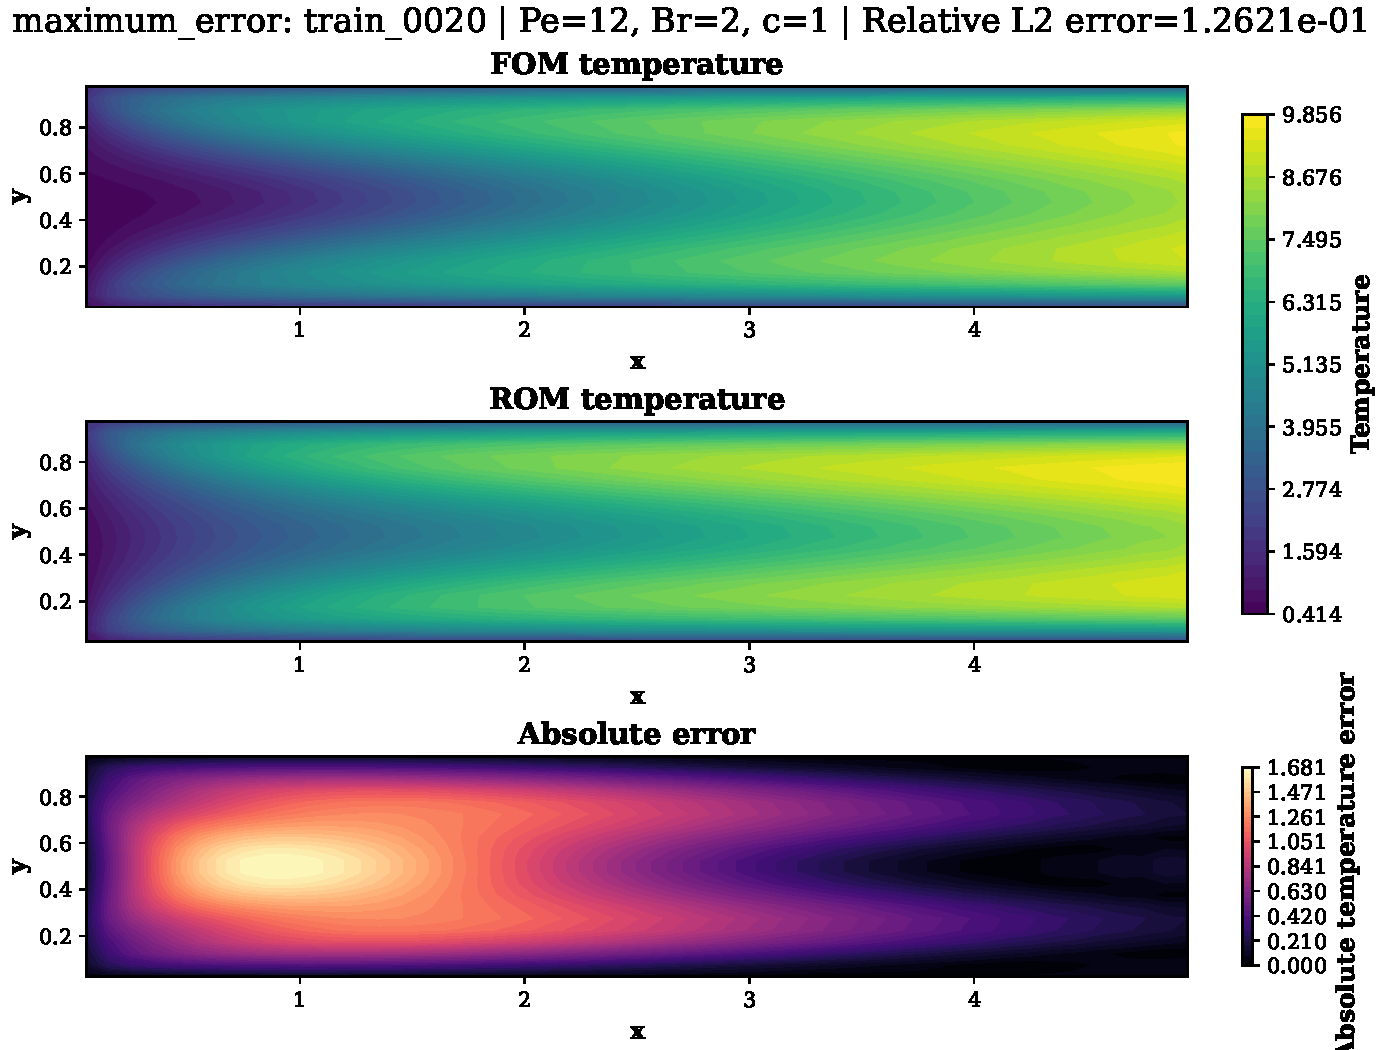
\includegraphics[width=\textwidth]
    {figures/Galerkin_maximum_error.pdf}
    \caption{Full-order temperature field, Galerkin ROM
    reconstruction, and corresponding error field for
    the maximum-error case (\texttt{train\_0020}).}
    \label{fig:galerkin_maximum_error}
\end{figure}


\subsection{Initial LHS evaluation and mode-count study}
\label{subsec:lhs_mode_count_results}

The first stage of ROM refinement examines the predictive
accuracy of the original POD basis using an independent
Latin hypercube sampling (LHS) dataset. This dataset
contains 100 parameter combinations within the prescribed
domain:
\[
1\leq\mu\leq100,
\qquad
0.01\leq Br\leq2.
\]
For each parameter combination, a full-order simulation
is performed to provide a reference temperature field.
The original POD basis is then evaluated using the
Galerkin reduced-order model.

The purpose of this evaluation is to identify the
dependence of ROM accuracy on the number of retained
POD modes and to locate regions of the parameter domain
where the original basis produces relatively large
errors. The resulting error records are subsequently
used to guide the selection of additional training
snapshots.

\paragraph{Effect of the retained basis dimension.}

The original POD basis is evaluated using the mode
counts
\[
r\in\{1,2,3,4,5,6,8,10\}.
\]
For each mode count, the first $r$ spatial modes are
retained, and the corresponding Galerkin reduced system
is solved for all 100 LHS cases. The relative $L_2$
error, RMSE, and maximum error are calculated for each
case. The aggregate statistics are reported in
Table~\ref{tab:lhs_mode_count_results}.

\begin{table}[htbp]
    \centering
    \caption{ROM error statistics for different retained
    POD mode counts over the 100 LHS screening cases.}
    \label{tab:lhs_mode_count_results}
    \scriptsize
    \setlength{\tabcolsep}{4pt}
    \begin{tabular}{ccccccc}
        \toprule
        \textbf{Modes} &
        \textbf{Cases} &
        \textbf{Mean error} &
        \textbf{Median error} &
        \textbf{95th percentile} &
        \textbf{Maximum error} &
        \textbf{Mean RMSE} \\
        \midrule
        1  & 100 & 0.395587 & 0.418291 & 0.614300 & 0.636144 & 0.813243 \\
        2  & 100 & 0.171552 & 0.175393 & 0.348644 & 0.410623 & 0.378429 \\
        3  & 100 & 0.027889 & 0.025590 & 0.063268 & 0.079345 & 0.073850 \\
        4  & 100 & 0.007663 & 0.006444 & 0.020409 & 0.044846 & 0.024056 \\
        5  & 100 & 0.002532 & 0.001145 & 0.013146 & 0.031450 & 0.010355 \\
        6  & 100 & 0.001377 & 0.000184 & 0.008551 & 0.024884 & 0.006698 \\
        8  & 100 & 0.000726 & $3.02\times10^{-6}$ & 0.005354 & 0.015513 & 0.003776 \\
        10 & 100 & 0.000468 & $2.96\times10^{-8}$ & 0.003338 & 0.010435 & 0.002440 \\
        \bottomrule
    \end{tabular}
\end{table}

The results show a substantial reduction in ROM error
as the number of retained modes increases. With one
mode, the mean relative $L_2$ error is approximately
39.56\%, and the maximum error reaches 63.61\%.
Increasing the basis dimension to three modes reduces
the mean error to 2.79\%. With four modes, the mean
error decreases further to approximately 0.77\%.

The improvement continues with additional modes.
For ten retained modes, the mean relative $L_2$ error
is approximately 0.0468\%, while the maximum error
decreases to approximately 1.04\%. The 95th-percentile
error also decreases from 61.43\% with one mode to
approximately 0.334\% with ten modes.

The median error at ten modes is particularly small,
approximately $2.96\times10^{-8}$. However, the
maximum error remains considerably larger than the
median. This indicates that the ROM does not achieve
uniformly similar accuracy across all parameter
combinations, even when a relatively large number
of modes is retained.

Figure~\ref{fig:mode_count_error_statistics} presents
the variation of the mean, median, 95th-percentile,
and maximum relative $L_2$ errors with the number of
retained modes.

\begin{figure}[htbp]
    \centering
    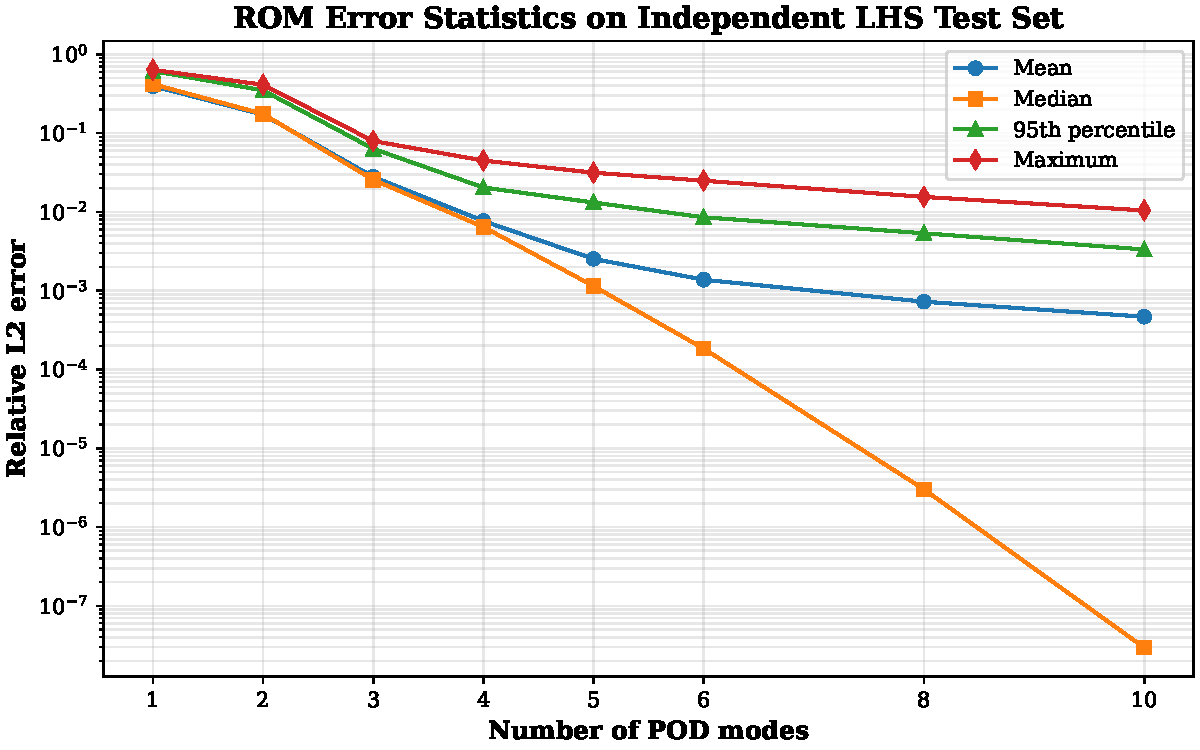
\includegraphics[width=0.95\textwidth]
    {figures/mode_count_study_error_statistics.pdf}
    \caption{Mean, median, 95th-percentile, and maximum
    relative $L_2$ errors as functions of the number
    of retained POD modes for the 100 LHS screening cases.}
    \label{fig:mode_count_error_statistics}
\end{figure}

The decreasing error statistics confirm that increasing
the reduced basis dimension improves the overall
accuracy of the original Galerkin ROM over the sampled
parameter domain. Nevertheless, the differences
between the median and maximum errors suggest that
some parameter regions remain more difficult to
represent than others. Therefore, increasing the
number of modes alone does not fully address the
spatially localized deficiencies of the original basis.

\paragraph{Error distribution in the parameter domain.}

To examine where the ROM produces relatively large
errors, the case-wise relative $L_2$ errors are also
visualized over the two-dimensional parameter space.
Each LHS case is associated with its parameter
coordinates $(\mu,Br)$ and its corresponding ROM
error.

Since the LHS parameter combinations are irregularly
distributed, they do not form a structured rectangular
grid. Therefore, a triangulation-based visualization
is used to represent the error distribution. The
sample points are connected through a triangular
mesh, and the error values are interpolated over the
resulting triangular regions to construct a
contour-like map.

Figure~\ref{fig:lhs_triangulated_error} presents
the resulting spatial distribution of the relative
$L_2$ error across the parameter domain.

\begin{figure}[htbp]
    \centering
    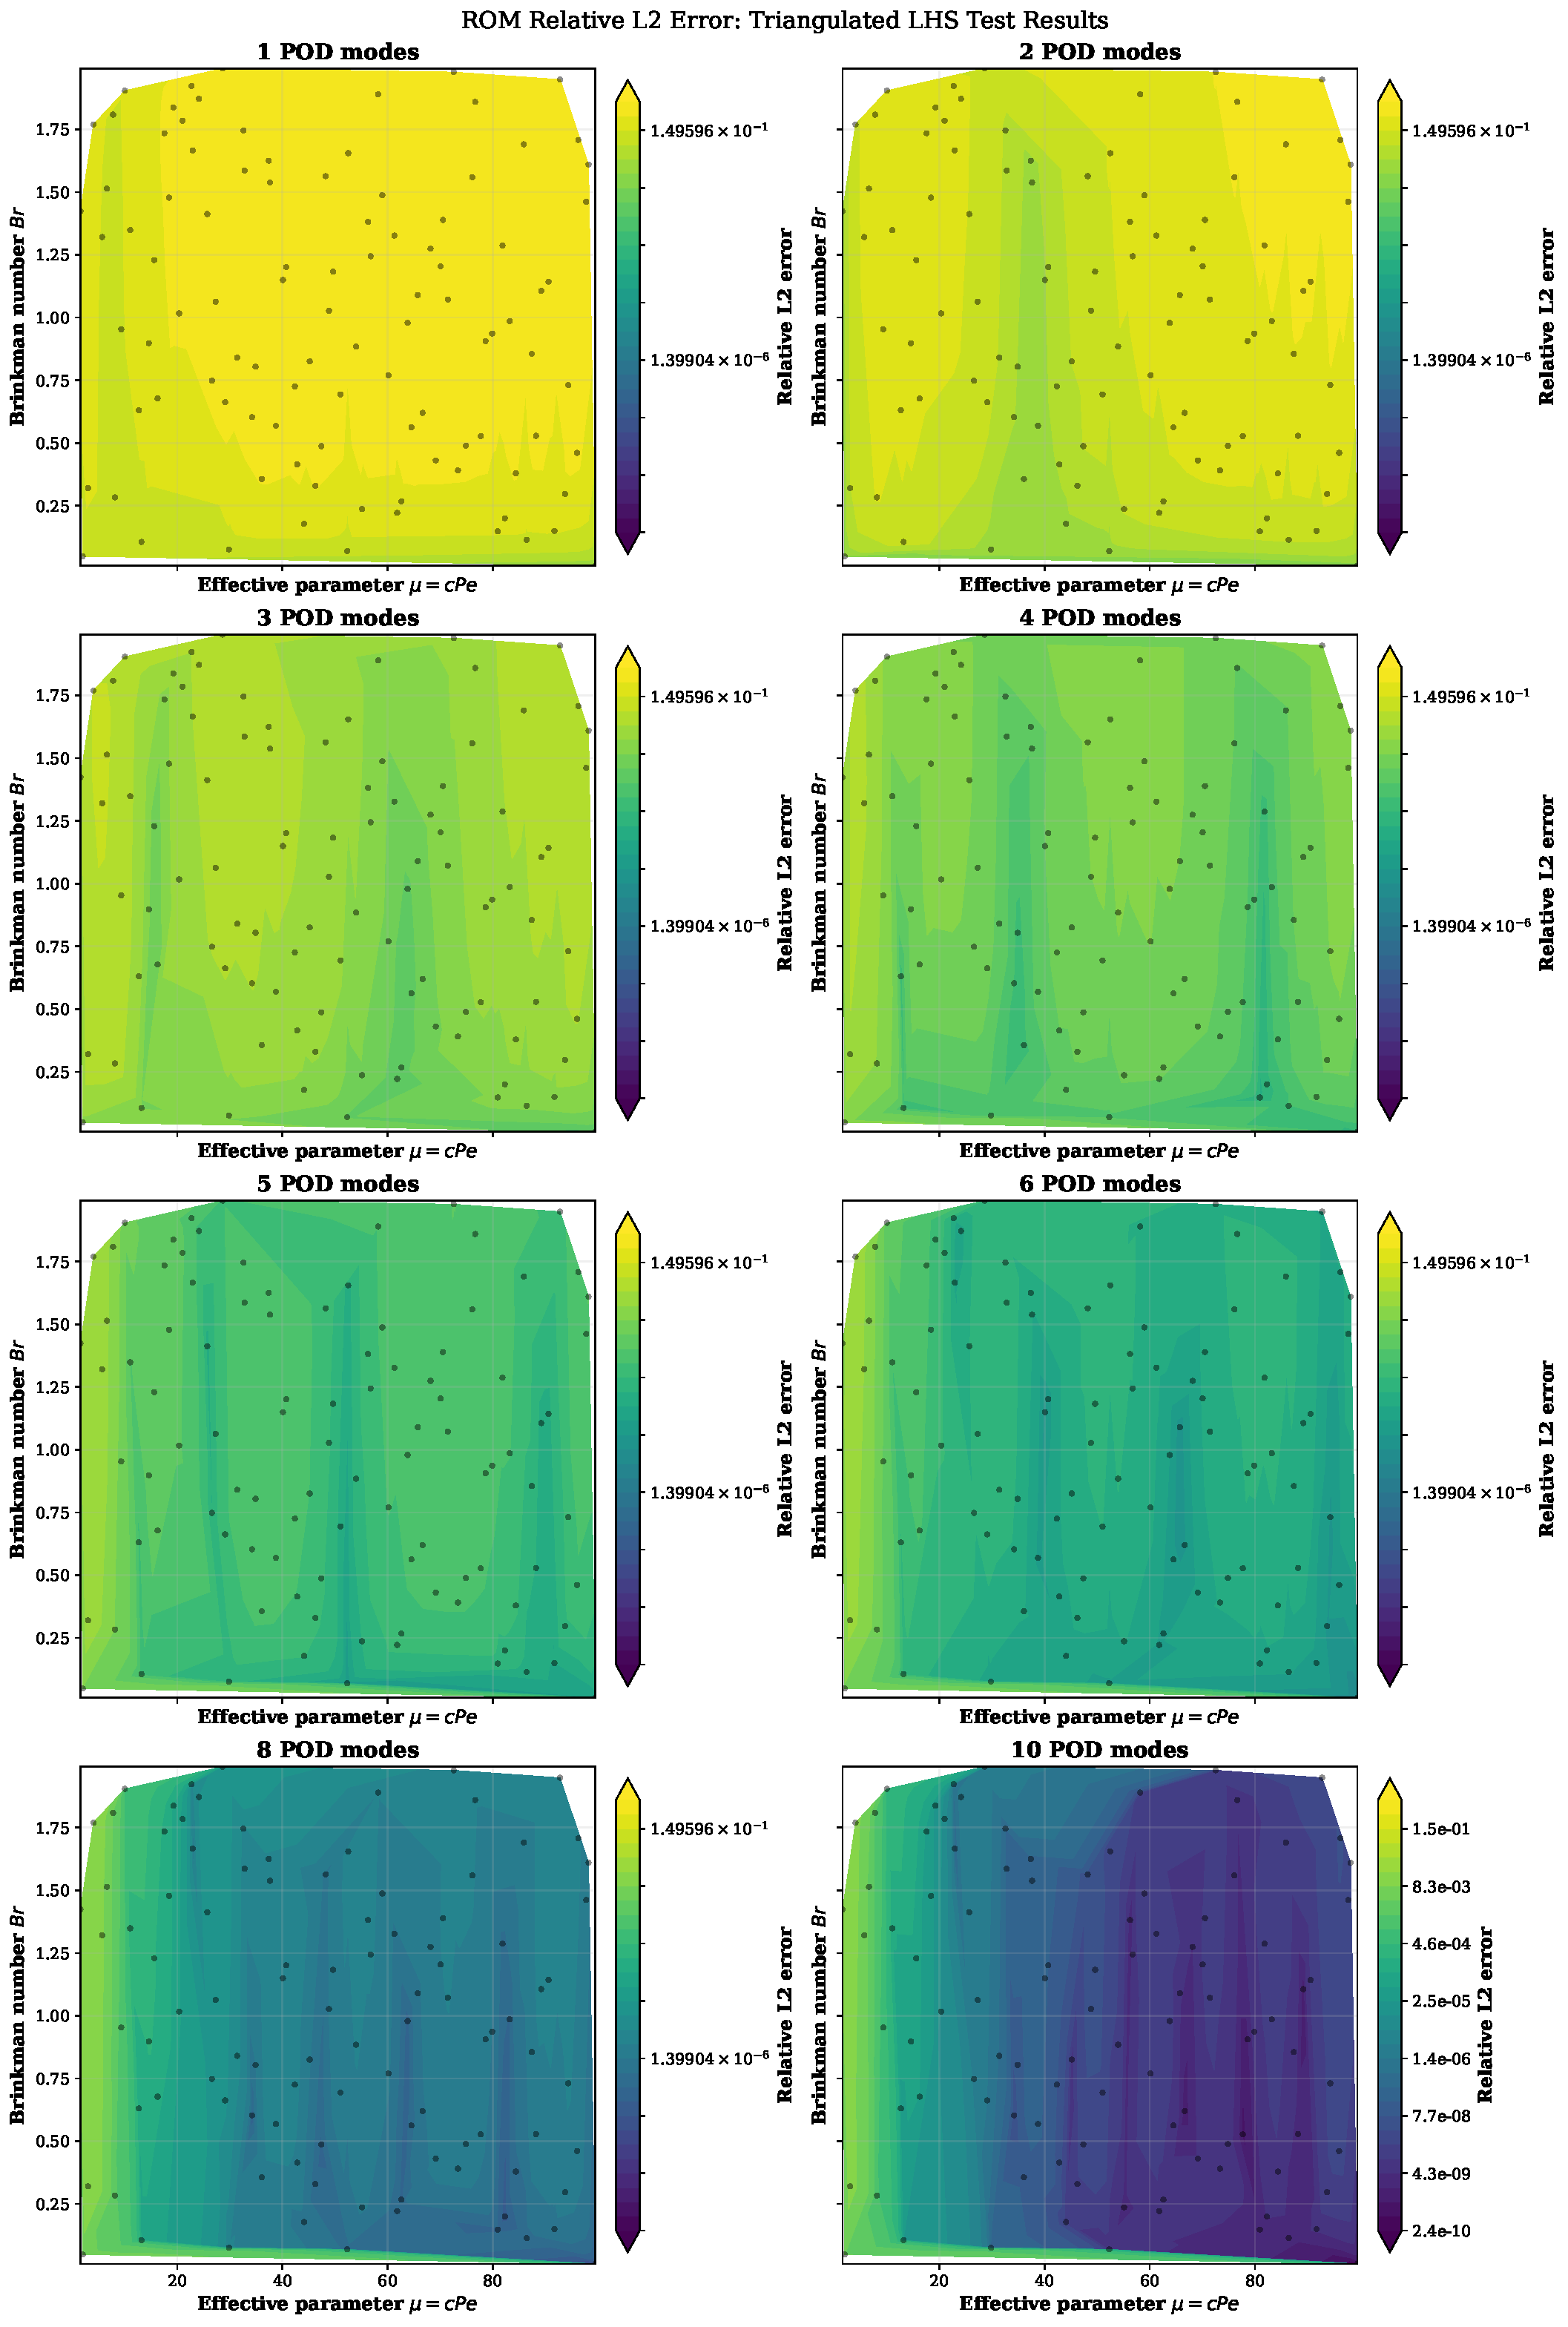
\includegraphics[width=0.95\textwidth]
    {figures/relative_l2_error_triangulated_lhs.pdf}
    \caption{Triangulation-based visualization of the
    relative $L_2$ ROM error over the 100 LHS
    parameter combinations.}
    \label{fig:lhs_triangulated_error}
\end{figure}

The triangulated map provides a visual representation
of the variation in ROM accuracy across the sampled
parameter domain. Regions associated with larger
errors can be identified and examined to determine
where additional training snapshots may be useful.
The interpolated regions are intended as a
visualization of the sampled error data; they do
not represent additional ROM evaluations between
the LHS points.

The mode-count statistics and parameter-space
visualization together provide the basis for the
subsequent snapshot-enrichment procedure. Rather than
increasing the training dataset uniformly, the
following refinement stage selects candidate
parameter combinations from the high-error cases
and generates additional full-order snapshots
around the selected locations.

\subsection{Snapshot enrichment and construction of the augmented basis}
\label{subsec:augmented_basis_results}

The high-error regions identified during the initial LHS
screening were used to generate additional full-order
snapshots. The hotspot-selection procedure identified
three parameter-space locations, around which local
parameter grids were constructed. After applying the
parameter-domain restrictions, removing duplicate
combinations, and excluding cases already present in
the original training grid, 15 additional parameter
combinations were obtained.

All 15 additional full-order simulations converged
successfully. No nonconverged cases or simulation
errors were reported. The resulting snapshot matrix
has dimensions $1000\times15$, as summarized in
Table~\ref{tab:enrichment_generation_results}.

\begin{table}[htbp]
    \centering
    \caption{Results of the additional snapshot-generation
    procedure.}
    \label{tab:enrichment_generation_results}
    \begin{tabular}{lc}
        \toprule
        \textbf{Quantity} & \textbf{Result} \\
        \midrule
        Selected hotspot centres & 3 \\
        Generated parameter combinations & 15 \\
        Successful full-order simulations & 15 \\
        Nonconverged simulations & 0 \\
        Cases with simulation errors & 0 \\
        Additional snapshot matrix dimensions & $1000\times15$ \\
        \bottomrule
    \end{tabular}
\end{table}

The additional snapshots were combined with the original
100 snapshots to construct the augmented snapshot matrix:
\[
\mathbf{X}_{\mathrm{aug}}
=
\begin{bmatrix}
\mathbf{X}_{\mathrm{original}} &
\mathbf{X}_{\mathrm{additional}}
\end{bmatrix}.
\]
Therefore,
\[
\mathbf{X}_{\mathrm{aug}}
\in\mathbb{R}^{1000\times115}.
\]
A new SVD was performed on this combined matrix, and
the augmented POD basis was obtained from its left
singular vectors.

The three-mode cumulative POD energy of the augmented
basis is 99.9699\%, compared with 99.9833\% for the
original basis. Although the augmented basis has a
slightly lower cumulative energy at this mode count,
this does not directly indicate poorer predictive
accuracy. The additional snapshots change the total
snapshot energy and its distribution among the modes.
The effect of enrichment must therefore be judged
through the subsequent ROM evaluation on independent
parameter combinations.

\subsection{Independent comparison of the original and augmented bases}
\label{subsec:original_augmented_comparison}

The final comparison was performed using a separate
set of 100 LHS parameter combinations. These cases
were generated after construction of the augmented
basis. Parameter combinations already present in
either the original or augmented training datasets
were excluded. The full-order solver was then executed
for each accepted test case to obtain its reference
temperature field.

Both POD bases were evaluated using exactly the same
100 test cases and the same eight retained mode counts:
\[
r\in\{1,2,3,4,5,6,8,10\}.
\]
For each test case and mode count, the original-basis
ROM and augmented-basis ROM were solved and compared
against the same full-order temperature field. This
resulted in
\[
2\times100\times8=1600
\]
ROM evaluations.

The comparison therefore changes the POD basis while
keeping the test cases, reference solutions, mode
counts, and error definitions fixed.

\paragraph{Comparison of aggregate error statistics.}

Table~\ref{tab:final_basis_error_statistics} reports
the relative $L_2$ error distributions for the two
bases. The mean, median, 95th-percentile, and maximum
errors are included for each retained mode count.

\begin{table}[htbp]
    \centering
    \caption{Relative $L_2$ error statistics for the
    original and augmented POD bases over 100 independent
    test cases.}
    \label{tab:final_basis_error_statistics}
    \scriptsize
    \setlength{\tabcolsep}{3pt}
    \resizebox{\textwidth}{!}{%
        \begin{tabular}{ccccccc}
            \toprule
            \textbf{Basis} &
            \textbf{Modes} &
            \textbf{Cases} &
            \textbf{Mean} &
            \textbf{Median} &
            \textbf{95th percentile} &
            \textbf{Maximum} \\
            \midrule
            Original  & 1  & 100 & 0.401768 & 0.437246 & 0.620615 & 0.634832 \\
            Original  & 2  & 100 & 0.176187 & 0.166973 & 0.371498 & 0.411629 \\
            Original  & 3  & 100 & 0.028506 & 0.024564 & 0.062156 & 0.081035 \\
            Original  & 4  & 100 & 0.008127 & 0.007205 & 0.026946 & 0.044410 \\
            Original  & 5  & 100 & 0.002725 & 0.001065 & 0.018959 & 0.030992 \\
            Original  & 6  & 100 & 0.001571 & 0.000189 & 0.013137 & 0.026048 \\
            Original  & 8  & 100 & 0.000876 & $3.00\times10^{-6}$ & 0.006426 & 0.018205 \\
            Original  & 10 & 100 & 0.000577 & $3.31\times10^{-8}$ & 0.003450 & 0.013008 \\
            \midrule
            Augmented & 1  & 100 & 0.384505 & 0.423167 & 0.594550 & 0.608058 \\
            Augmented & 2  & 100 & 0.193602 & 0.163706 & 0.435441 & 0.468897 \\
            Augmented & 3  & 100 & 0.036678 & 0.035301 & 0.079193 & 0.095283 \\
            Augmented & 4  & 100 & 0.013629 & 0.013465 & 0.028654 & 0.037714 \\
            Augmented & 5  & 100 & 0.003841 & 0.004188 & 0.007181 & 0.009805 \\
            Augmented & 6  & 100 & 0.000930 & 0.000758 & 0.001740 & 0.005040 \\
            Augmented & 8  & 100 & 0.000141 & 0.000123 & 0.000241 & 0.001747 \\
            Augmented & 10 & 100 & $1.74\times10^{-5}$ & $1.30\times10^{-5}$ & $3.07\times10^{-5}$ & 0.000401 \\
            \bottomrule
        \end{tabular}%
    }
\end{table}

For one retained mode, the augmented basis reduces
the mean relative $L_2$ error from 0.401768 to
0.384505. The improvement is modest, but it is
observed across all 100 test cases.

For two and three modes, however, the augmented basis
produces higher mean and maximum errors. The mean
relative $L_2$ error increases from 0.176187 to
0.193602 for two modes and from 0.028506 to 0.036678
for three modes. The maximum errors also increase
at both ranks.

A similar increase in mean error occurs for four
and five modes. However, the maximum error decreases
at both mode counts. For four modes, it decreases
from 0.044410 to 0.037714. For five modes, it
decreases more substantially, from 0.030992 to
0.009805. Thus, the enrichment reduces the largest
observed errors at these ranks, although the mean
error becomes higher.

The behavior changes at six modes. The augmented
basis reduces the mean relative $L_2$ error from
0.001571 to 0.000930 and the maximum error from
0.026048 to 0.005040. These reductions become
more pronounced at eight and ten modes.

At ten modes, the mean relative $L_2$ error decreases
from 0.000577 to $1.74\times10^{-5}$, while the
maximum error decreases from 0.013008 to 0.000401.
The corresponding reductions are approximately
96.98\% and 96.92\%, respectively. The 95th-percentile
error also decreases from 0.003450 to
$3.07\times10^{-5}$.

\paragraph{Paired case-wise comparison.}

The aggregate statistics do not indicate how
consistently the augmented basis improves individual
test cases. For this reason, the error difference
is calculated separately for every paired case:
\[
\boxed{
\Delta\epsilon_k
=
\epsilon_{\mathrm{rel},k}^{\mathrm{aug}}
-
\epsilon_{\mathrm{rel},k}^{\mathrm{orig}}.
}
\]
A negative value indicates that the augmented basis
produces a lower error, while a positive value
indicates that the original basis performs better.

The percentage of improved cases is calculated as
\[
P_{\mathrm{improved}}
=
\frac{
N(\Delta\epsilon_k<0)
}{100}
\times100.
\]
The percentage reductions in mean and maximum errors
are also calculated relative to the original basis.

The paired results are summarized in
Table~\ref{tab:paired_enrichment_results}.

\begin{table}[htbp]
    \centering
    \caption{Paired comparison of the original and
    augmented POD bases over 100 independent test cases.}
    \label{tab:paired_enrichment_results}
    \scriptsize
    \setlength{\tabcolsep}{3pt}
    \resizebox{\textwidth}{!}{%
        \begin{tabular}{ccccccccc}
            \toprule
            \textbf{Modes} &
            \textbf{Mean reduction (\%)} &
            \textbf{Max. reduction (\%)} &
            \textbf{Mean $\Delta\epsilon$} &
            \textbf{Median $\Delta\epsilon$} &
            \textbf{5th percentile} &
            \textbf{95th percentile} &
            \textbf{Improved cases (\%)} \\
            \midrule
            1  & 4.2967   & 4.2175   & -0.017260 & -0.017340 & -0.026400 & -0.004820 & 100 \\
            2  & -9.8843  & -13.9125 & 0.017415  & 0.041945  & -0.080070 & 0.077803  & 33 \\
            3  & -28.6650 & -17.5825 & 0.008171  & 0.011487  & -0.027850 & 0.031049  & 32 \\
            4  & -67.6905 & 15.0773  & 0.005501  & 0.007381  & -0.014240 & 0.021053  & 28 \\
            5  & -40.9432 & 68.3639  & 0.001116  & 0.002426  & -0.013540 & 0.005900  & 22 \\
            6  & 40.7665  & 80.6523  & -0.000640 & 0.000445  & -0.011450 & 0.001546  & 22 \\
            8  & 83.9121  & 90.4018  & -0.000730 & 0.000082  & -0.006310 & 0.000193  & 11 \\
            10 & 96.9841  & 96.9175  & -0.000560 & 0.00000833 & -0.003440 & 0.0000271 & 20 \\
            \bottomrule
        \end{tabular}%
    }
\end{table}

For one mode, all test cases improve with the augmented
basis. At two through five modes, the percentage of
improved cases decreases to between 22\% and 33\%.
The positive mean and median case-wise error changes
at these ranks indicate that the augmented basis
generally produces higher errors across the paired
test cases, even though the maximum error is reduced
at four and five modes.

At six, eight, and ten modes, the mean case-wise
error change becomes negative, indicating an overall
reduction when the differences are averaged. However,
the median case-wise change remains positive at all
three mode counts, and the percentage of improved
cases is only 22\%, 11\%, and 20\%, respectively.

This distinction is important. At eight modes, for
example, the mean relative $L_2$ error is reduced
by approximately 83.91\%, yet only 11 of the 100
test cases have lower errors with the augmented
basis. At ten modes, the mean error is reduced by
approximately 96.98\%, while only 20 cases improve.

Therefore, the large reductions in aggregate errors
are concentrated in a relatively small number of
test cases. The errors of the remaining cases
generally increase, but these increases are
outweighed by substantial reductions in a smaller
number of cases. This explains why the mean and
maximum errors can improve while most individual
cases do not.

\paragraph{Spatial distribution of the error changes.}

The paired error distributions are also examined
over the parameter domain. The triangulated error
maps compare the relative $L_2$ errors of the
original and augmented bases at each retained
mode count. These maps help identify whether the
changes in the aggregate statistics are associated
with the parameter regions targeted during
snapshot enrichment.

The error-statistics comparison is shown in
Figure~\ref{fig:original_augmented_error_statistics}.
The corresponding relative error reductions are
shown in Figure~\ref{fig:original_augmented_error_reduction}.

\begin{figure}[htbp]
    \centering
    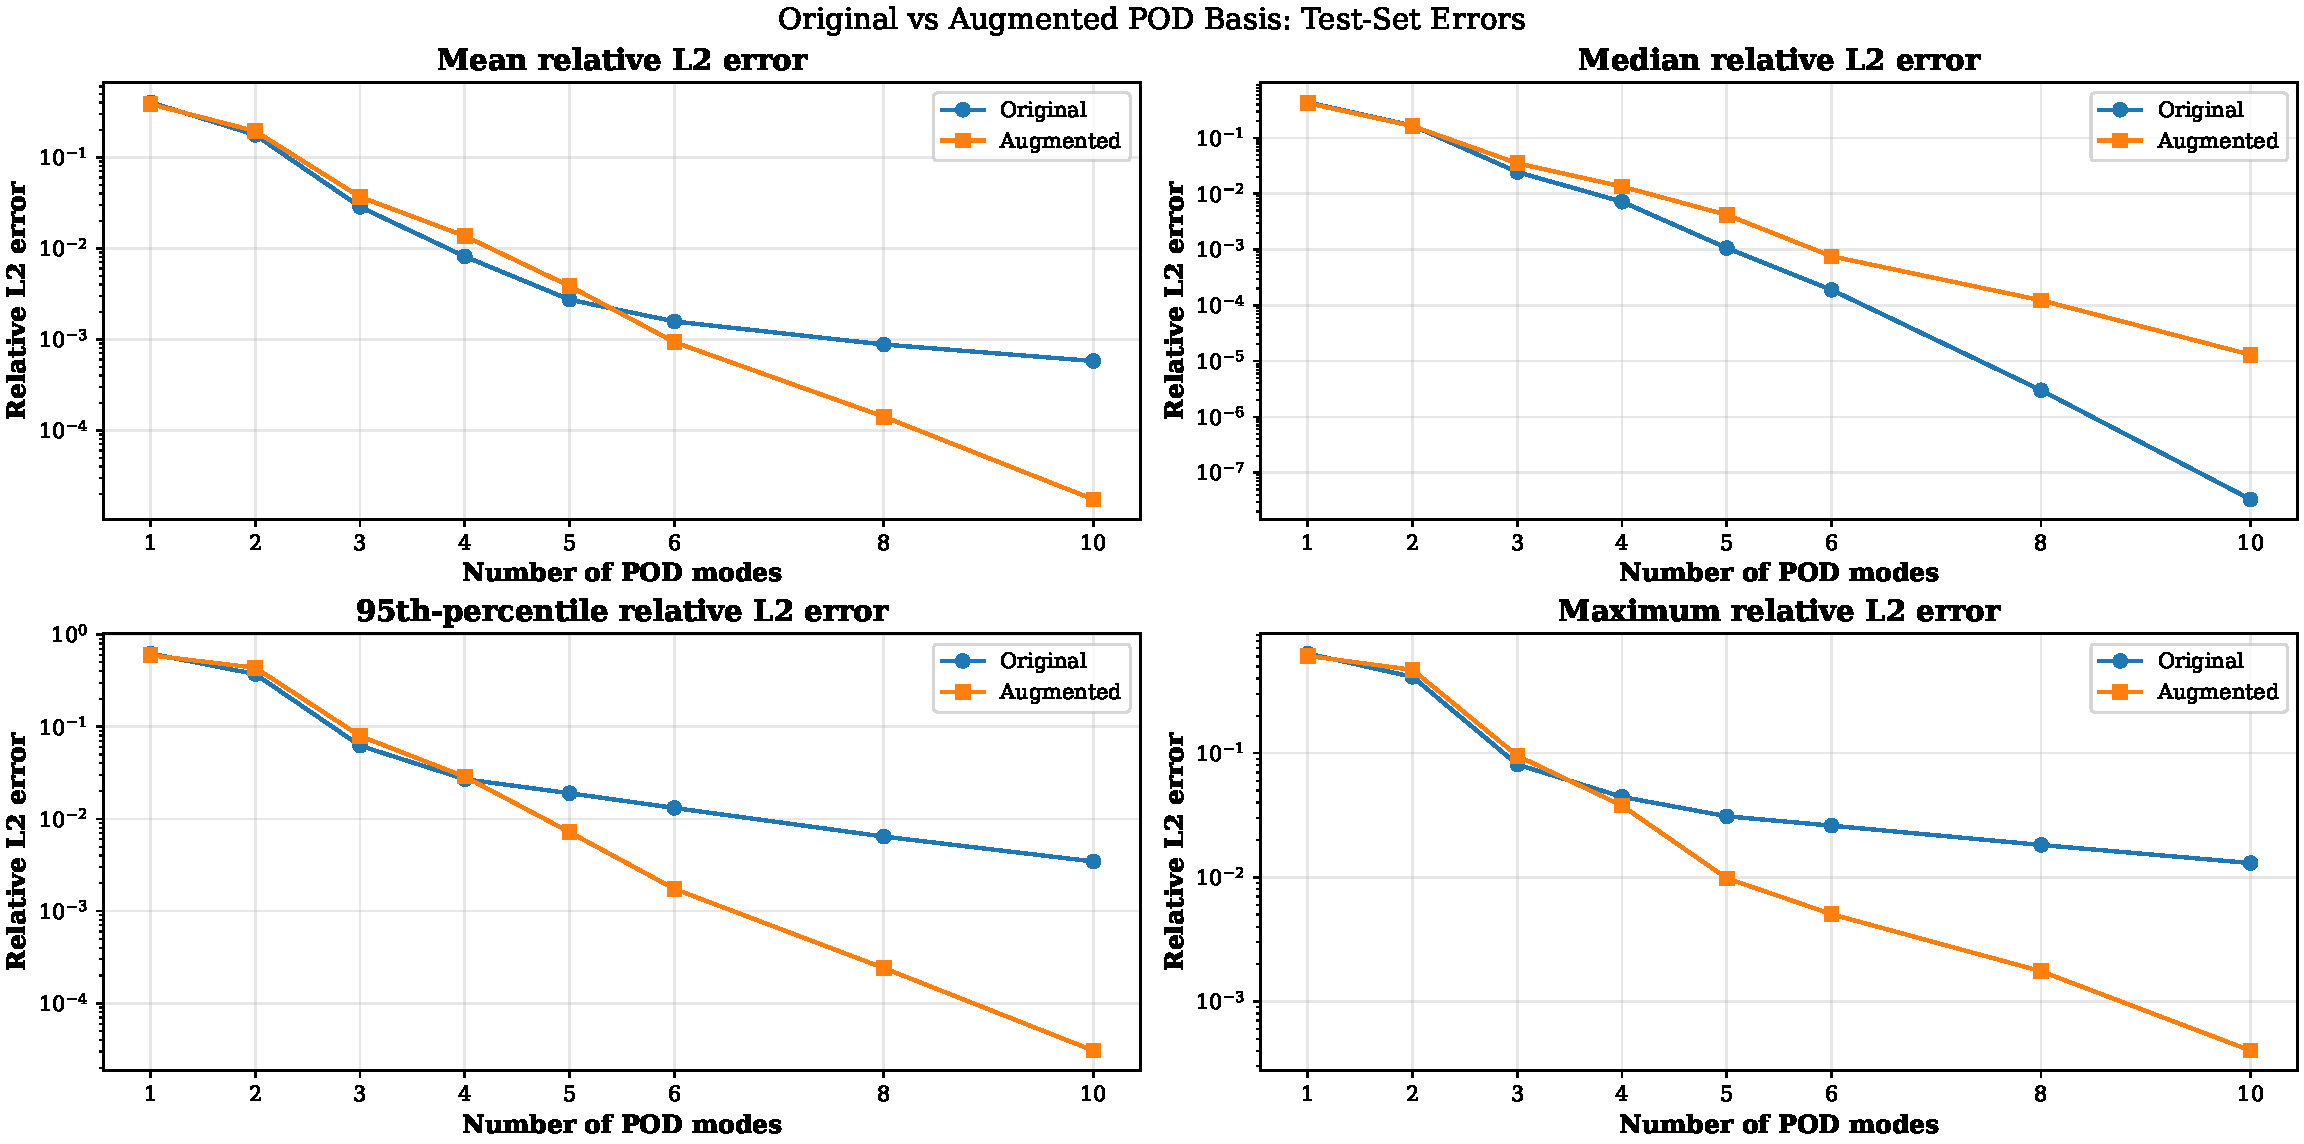
\includegraphics[width=0.95\textwidth]
    {figures/original_augmented_rom_comparison_error_statistics.pdf}
    \caption{Comparison of error statistics for the
    original and augmented POD bases across the
    retained mode counts.}
    \label{fig:original_augmented_error_statistics}
\end{figure}

\begin{figure}[htbp]
    \centering
    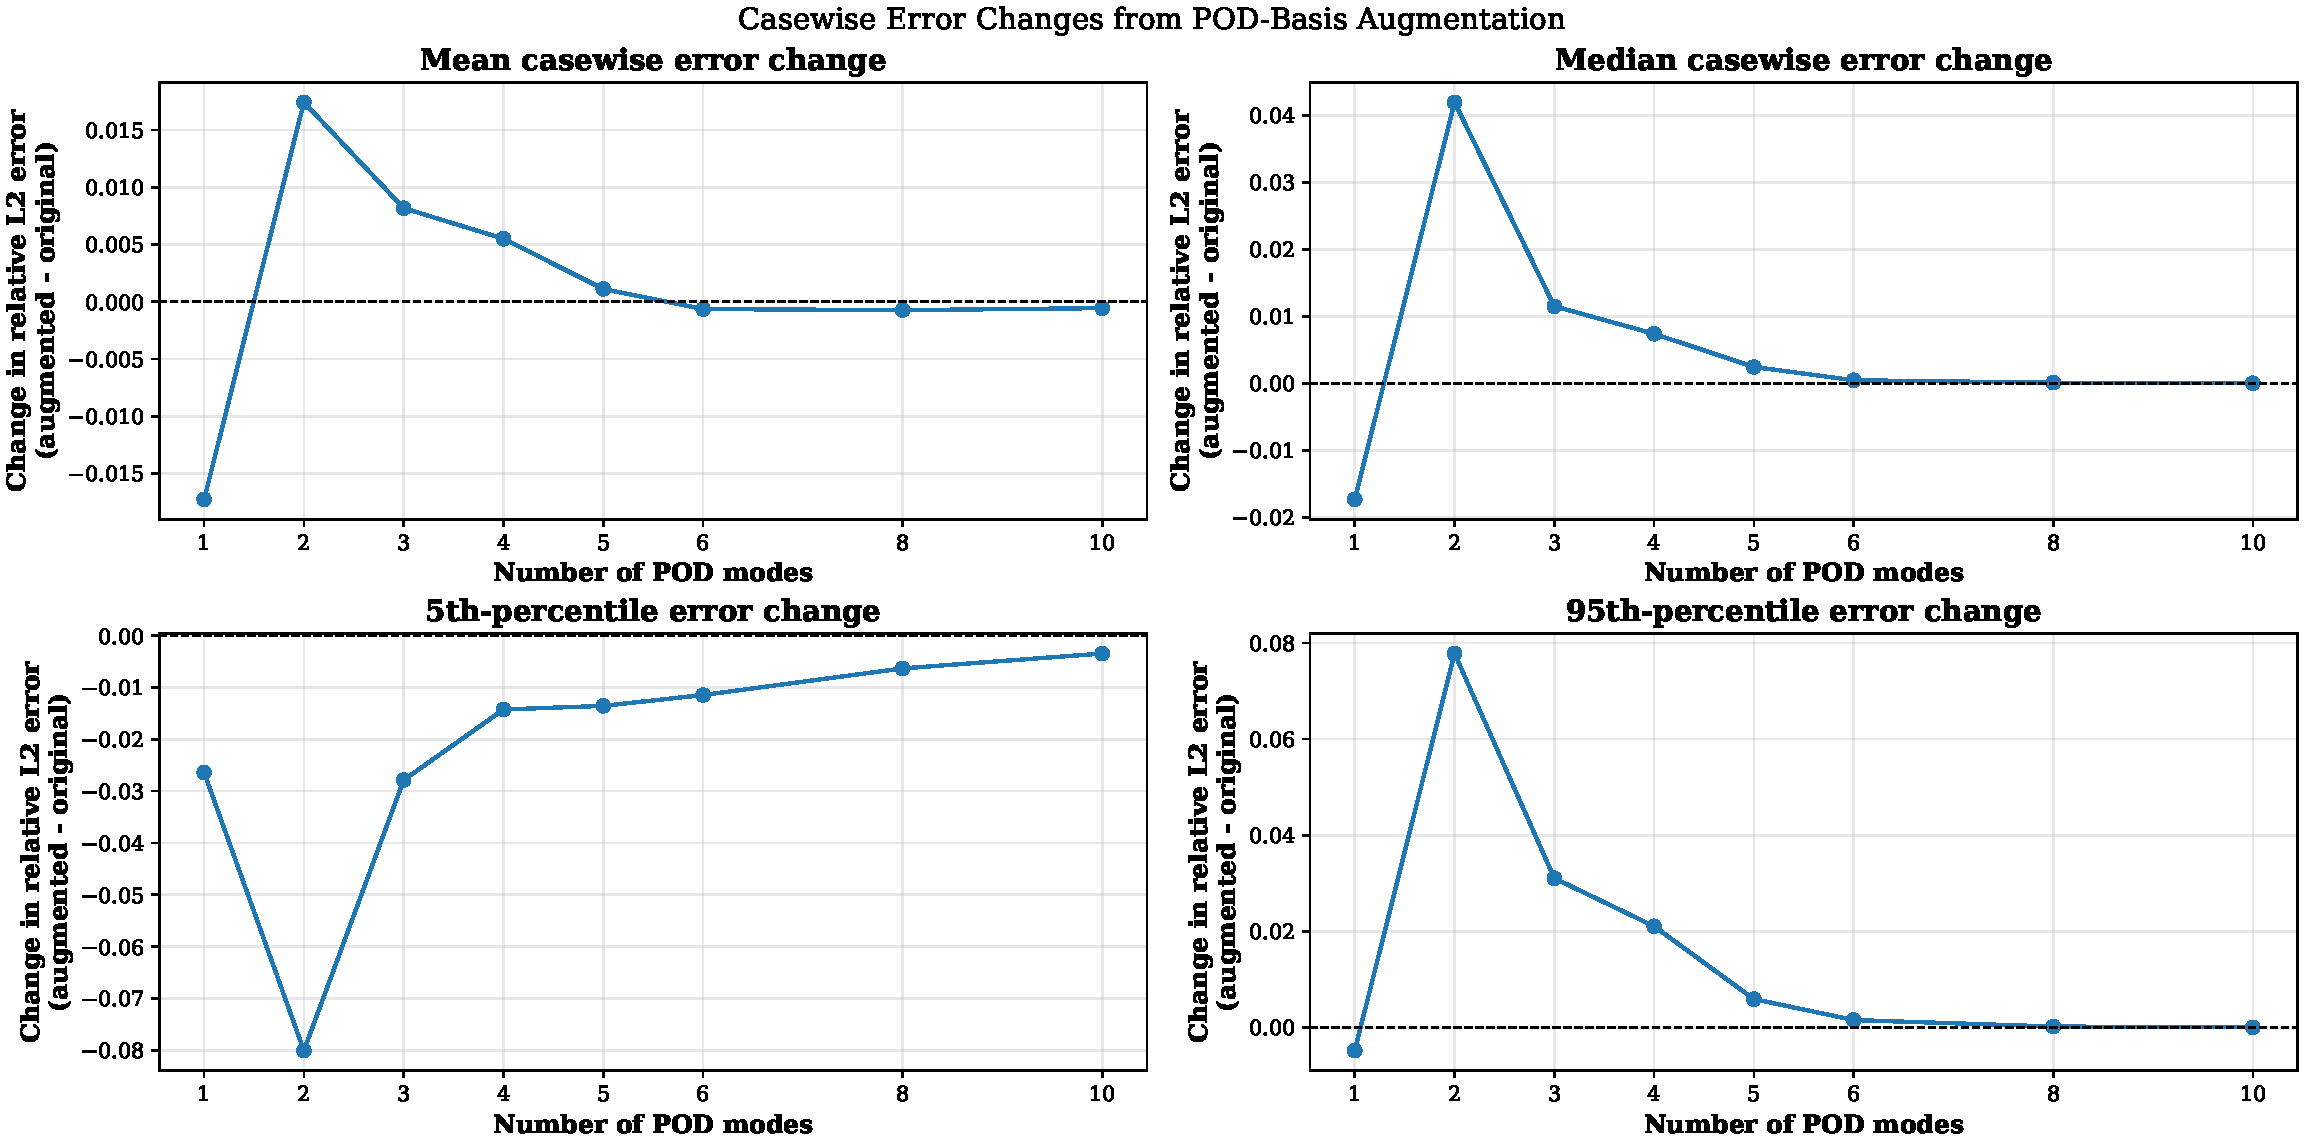
\includegraphics[width=0.95\textwidth]
    {figures/original_augmented_rom_comparison_error_reduction.pdf}
    \caption{Relative error reductions obtained with
    the augmented POD basis compared with the
    original basis for different retained mode counts.}
    \label{fig:original_augmented_error_reduction}
\end{figure}

The parameter-space error maps provide a more
localized comparison. In particular, the ten-mode
comparison is shown in
Figure~\ref{fig:augmented_error_map_ten_modes}.

\begin{figure}[htbp]
    \centering
    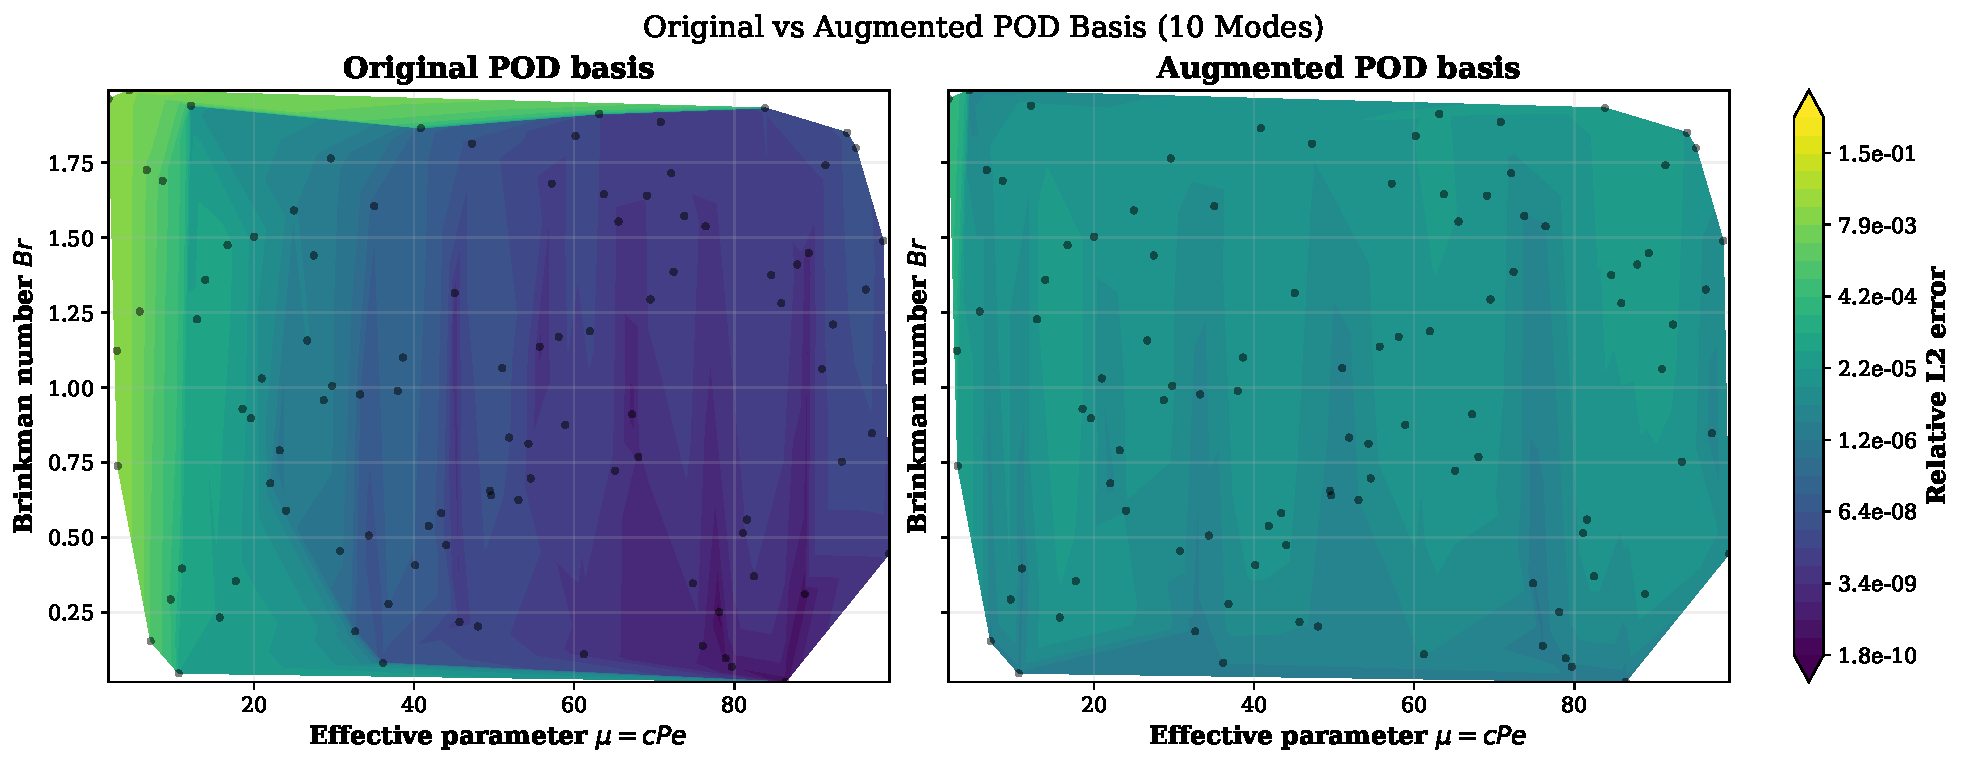
\includegraphics[width=0.95\textwidth]
    {figures/error_map_10_modes.pdf}
    \caption{Triangulated comparison of the original
    and augmented ROM relative $L_2$ errors over
    the independent test parameter domain for
    ten retained modes.}
    \label{fig:augmented_error_map_ten_modes}
\end{figure}

The error maps should be interpreted together with
the paired statistics. They show how the changes
in prediction error are distributed over the
parameter domain, whereas the aggregate statistics
describe their overall magnitude. The reduction
in the largest errors at higher mode counts is
consistent with the purpose of the targeted
enrichment: adding snapshots near parameter regions
where the original basis had difficulty representing
the solution.

\paragraph{Additional error measures and computational time.}

The RMSE and maximum absolute error provide further
information about the temperature-field differences.
For ten modes, the mean RMSE decreases from
$3.786\times10^{-3}$ to $7.24\times10^{-5}$.
The maximum absolute error over all test cases
decreases from 0.434450 to 0.014533.

The mean ROM computation times are also compared.
For the original basis, they range from approximately
$3.07\times10^{-4}$ to
$5.15\times10^{-4}$ seconds per case. For the
augmented basis, they range from approximately
$3.07\times10^{-4}$ to
$7.05\times10^{-4}$ seconds per case. These
measurements indicate a small increase in evaluation
time for most of the higher mode counts. However,
the times remain sub-millisecond, and the differences
should be interpreted with care because of their
small magnitude.

\paragraph{Overall discussion.}

The snapshot-enrichment procedure successfully
increased the training dataset from 100 to 115
full-order snapshots, with all additional simulations
converging. The independent paired evaluation shows
that the resulting augmented basis does not improve
the ROM uniformly across the parameter domain.

At low and intermediate mode counts, the augmented
basis generally produces higher mean errors, although
the maximum errors decrease at four and five modes.
At six, eight, and ten modes, both the mean and
maximum errors decrease substantially. The
ten-mode results are particularly pronounced, with
approximately 97\% reductions in both quantities.

However, the percentage of improved individual
test cases remains low at these higher mode counts.
In particular, only 20\% of the cases improve at
ten modes. This indicates that the enrichment
strongly improves a limited set of parameter
combinations, while it slightly degrades the
approximation for many others.

The results therefore suggest that local snapshot
enrichment is effective at reducing the large
errors associated with selected regions of the
parameter domain, but does not necessarily improve
the global approximation uniformly. The augmented
basis changes the distribution of spatial modes,
and the effect of this change depends on the
retained basis dimension and the parameter
combination being evaluated.

For the present enrichment strategy, the main
benefit is a substantial reduction in the upper
end of the error distribution at higher mode
counts, rather than a consistent improvement for
every test case. Further refinement would therefore
need to consider both the high-error regions and
the broader parameter-space accuracy when selecting
additional snapshots.


\subsection{Computational cost}
\label{subsec:computational_cost}

The Galerkin--POD formulation reduces the dimension of
the governing system from the original full-order spatial
dimension to the number of retained POD modes. For the
present computational grid, the full-order temperature
field contains
\[
N=N_xN_y=50\times20=1000
\]
physical degrees of freedom. In the three-mode
configuration considered here, the reduced system
contains only three unknown modal coefficients:
\[
\mathbf{A}_r\mathbf{a}=\mathbf{b}_r,
\qquad
\mathbf{a}\in\mathbb{R}^{3}.
\]
Thus, the reduced linear system has only three unknowns,
compared with the 1000 unknowns of the full-order
spatial problem. This corresponds to a 99.7\% reduction
in the number of system unknowns.

After solving the reduced system, the complete
temperature field is reconstructed through
\[
\boxed{
\mathbf{T}_{\mathrm{ROM}}
=
\mathbf{T}_{\mathrm{ref}}+\mathbf{V}_3\mathbf{a}.
}
\]
Although the reduced solve involves only three
coefficients, the reconstruction still produces
a temperature vector with 1000 physical values.

\paragraph{Full-order and reduced-order computation times.}

The recorded computation times for the 100 full-order
training cases and the corresponding reduced-order
evaluations are summarized in
Table~\ref{tab:computational_time_comparison}.
The ROM calculations use three retained POD modes.

\begin{table}[htbp]
    \centering
    \caption{Recorded full-order and reduced-order
    computation times for the three-mode ROM.}
    \label{tab:computational_time_comparison}
    \begin{tabular}{lccccc}
        \toprule
        \textbf{Model} &
        \textbf{Cases} &
        \textbf{Mean (s)} &
        \textbf{Median (s)} &
        \textbf{Minimum (s)} &
        \textbf{Maximum (s)} \\
        \midrule
        FOM & 100 & 0.137740 & 0.136677 & 0.099995 & 0.218700 \\
        ROM & 99  & 0.054623 & 0.050581 & 0.046414 & 0.122380 \\
        \bottomrule
    \end{tabular}
\end{table}

The mean recorded full-order computation time is
approximately 0.138~s per case. The mean of the
99 supplied ROM timing records is approximately
0.0546~s. The corresponding median times are
approximately 0.1367~s and 0.0506~s, respectively.

The timing records therefore indicate that the
reduced-order calculations require less computation
time per case than the full-order simulations.
However, one ROM timing entry is missing from the
provided dataset. Consequently, the two reported
means are based on different numbers of records,
and a definitive paired speedup ratio is not
reported here.

\paragraph{Operator construction and reduced-system evaluation.}

The total computational cost of the ROM can be
separated into operator construction, Galerkin
projection, reduced-system solution, and temperature
reconstruction:
\[
\begin{aligned}
t_{\mathrm{ROM}}
={}&t_{\mathrm{operators}}
+t_{\mathrm{projection}}\\
&+t_{\mathrm{reduced\ solve}}
+t_{\mathrm{reconstruction}}.
\end{aligned}
\]

The operator-construction stage includes the assembly
of the full-order convection and diffusion matrices,
the viscous-dissipation source, and the lifting
contribution. These quantities are then projected
onto the retained POD basis.

The reduced-system evaluation stage consists of
assembling the parameter-dependent reduced matrix
and right-hand-side vector, solving the resulting
$3\times3$ linear system, and reconstructing the
temperature field.

For a fixed computational grid and prescribed
velocity field, the full-order spatial operators
and viscous-dissipation source are independent of
the parameter values. Their reduced projections
can therefore be constructed once and reused for
multiple parameter combinations. This would allow
the operator construction and projection costs to
be treated as an offline computational stage,
while the reduced-system solution and reconstruction
would form the online stage.

However, the current implementation reconstructs
the full-order operator components for individual
parameter cases before performing the reduced
projection and solution. Therefore, the current
workflow does not yet fully exploit the potential
offline-online separation.

The timing summary provided here contains the
overall FOM and ROM computation times, but does
not provide the numerical breakdown of operator
construction, projection, reduced-system solution,
and reconstruction. These contributions should
be reported separately using their respective
timing records. In particular, the reduced linear
solve time alone should not be interpreted as the
complete ROM evaluation time.

A consistent comparison of computational
efficiency should include all operations required
to produce the reconstructed ROM temperature
field and compare them with the complete
full-order solution process. Any one-time
preprocessing cost should be reported separately
from the per-parameter evaluation cost.

\subsection{Limitations}
\label{subsec:limitations}

The present reduced-order model has several limitations.
First, the velocity field is prescribed and remains fixed;
therefore, the model does not account for changes in the
flow field or flow-temperature coupling. The parameter
study is restricted to $\mu$ and $Br$, with $c=1$.
Furthermore, all simulations use a fixed $50\times20$
computational grid, and the final ROM represents only
steady-state solutions.

The snapshot-enrichment strategy also depends on the
high-error regions identified in the initial LHS
screening dataset. Consequently, the selected hotspots
reflect the behavior of the original ROM over that
particular sample. The augmented basis does not improve
the accuracy uniformly: its effect depends on the
retained mode count and parameter combination.

Although the final 100-case test dataset excludes
parameter combinations used in the original and
augmented training datasets, its complete independence
from the initial screening dataset should also be
confirmed. Since the screening results were used to
select the enrichment locations, any overlap with the
final test set could affect the interpretation of the
comparison. Therefore, claims about generalization
should be limited to the evaluated parameter domain
and supported by a check for overlap with both the
training and screening datasets.
